\documentclass[aspectratio=169,10pt]{beamer}
\usetheme{Madrid}
\usecolortheme{seahorse}
\usefonttheme{professionalfonts}

\setbeamertemplate{footline}[frame number]
\setbeamertemplate{navigation symbols}{}

\graphicspath{{figures/}}

\usepackage{amsmath,amssymb,amsthm}
\usepackage{graphicx}
\usepackage{listings}
\usepackage{xcolor}
\usepackage{booktabs}
\usepackage{tikz}
\usetikzlibrary{arrows.meta,positioning}

\lstset{
  basicstyle=\ttfamily\scriptsize,
  numbers=left,
  numberstyle=\tiny,
  frame=single,
  backgroundcolor=\color{gray!7},
  commentstyle=\color{green!50!black}\itshape,
  keywordstyle=\color{blue!70!black}\bfseries,
  stringstyle=\color{orange!70!black},
  breaklines=true,
  showstringspaces=false,
  language=Python
}

\newtheorem{axiomthm}{Axiom}

\title[UAI -- Ch.2.2]{An Introduction to Universal Artificial Intelligence}
\subtitle{Chapter 2: Background --- Section 2.2 \\ Measure Theory and Probability Theory}
\author{Based on Marcus Hutter, Elliot Catt, David Quarel (2024)}
\date{}

\begin{document}

% ==========================================================================
\begin{frame}
\titlepage
\end{frame}

% ==========================================================================
\begin{frame}{Outline}
\tableofcontents
\end{frame}

% ==========================================================================
\section{2.2.1 The Axioms of Probability Theory}

\begin{frame}{Why probability theory, with minimal measure theory?}
This section builds a working understanding of probability theory from four
axioms, and derives from them all the familiar properties (the chain rule
$\mathrm{P}(A,B)=\mathrm{P}(A|B)\mathrm{P}(B)$, expectations $\mathbb{E}[X]$,
independence, and so on) as theorems rather than assumptions. We only reach
for the underlying \emph{measure theory} --- the rigorous mathematics of
assigning ``sizes'' to sets --- when it is unavoidable, most notably when we
discuss convergence of random variables later in this chapter.

\vspace{2mm}
Throughout, we use $\mathbb{P}$ for probability, $\mathbb{E}$ for
expectation, $\mathbb{R}$ for the real numbers, $\mathbb{N}$ for the natural
numbers, and $\mathbb{B}=\{0,1\}$ for bits.
\end{frame}

\begin{frame}{Definition 2.2.1: $\sigma$-algebra}
\begin{block}{Definition 2.2.1 ($\sigma$-algebra)}
Given a set $\Omega$ (whose elements are called \emph{outcomes}), a
collection $\mathcal{F}$ of subsets of $\Omega$ is called a
\emph{$\sigma$-algebra} if it satisfies:
\begin{enumerate}
\item $\emptyset \in \mathcal{F}$.
\item If $A_1,A_2,\ldots \in \mathcal{F}$, then $\bigcup_{n=1}^{\infty}A_n \in \mathcal{F}$. (Closed under countable union)
\item If $A \in \mathcal{F}$, then $\Omega\setminus A =: A^c \in \mathcal{F}$. (Closed under complement)
\end{enumerate}
\end{block}
\textbf{Plain English.} $\Omega$ (capital omega) is the set of every possible
outcome of an experiment. $\mathcal{F}$ (script F) is a chosen collection of
subsets of $\Omega$ --- the subsets we are willing to call ``events'' and
assign a probability to. The three rules say: the impossible event must be
allowed, taking a union of countably many allowed events must again be
allowed, and the complement (``everything except'') of an allowed event must
be allowed. By De Morgan's law $\bigcap_{n=1}^{\infty}A_n = \big(\bigcup_{n=1}^{\infty}A_n^c\big)^c$,
a $\sigma$-algebra is automatically closed under countable intersection too.
\end{frame}

\begin{frame}{Measurable spaces, and the axioms of a probability measure}
\begin{block}{Definition 2.2.2 (Measurable space)}
A \emph{measurable space} is a pair $(\Omega,\mathcal{F})$ where $\mathcal{F}$
is a $\sigma$-algebra on $\Omega$.
\end{block}
We call $\Omega$ the \emph{sample space}, $\mathcal{F}$ the \emph{event
space}, and a set $A$ in the event space $\mathcal{F}$ an \emph{event}.

\begin{block}{Axiom 2.2.3 (Probability (semi)measure)}
A \emph{probability measure} (or measure) $\mathrm{P}$ on a measurable space
$(\Omega,\mathcal{F})$ is a function $\mathrm{P}:\mathcal{F}\to[0,1]$
satisfying:
\begin{enumerate}
\item $\mathrm{P}(\Omega) = 1$.
\item For any sequence of pairwise disjoint events $A_1,A_2,\ldots \in \mathcal{F}$ (i.e.\ $i\neq j \Rightarrow A_i\cap A_j=\emptyset$),
\[ \mathrm{P}\Big(\bigcup_{i=1}^{\infty}A_i\Big) = \sum_{i=1}^{\infty}\mathrm{P}(A_i) \]
\end{enumerate}
\end{block}
\textbf{Plain English.} $\mathrm{P}$ assigns to every event a number in
$[0,1]$: the event containing everything ($\Omega$) always has probability 1
(``certainty''), and if you break an event into countably many
non-overlapping pieces, the probability of the whole equals the sum of the
probabilities of the pieces.
\end{frame}

\begin{frame}{Weakening the axioms: semimeasures}
\begin{block}{Axiom 2.2.3 (continued): semi-probability and semimeasures}
\begin{enumerate}
\setcounter{enumi}{2}
\item If we weaken Axiom 1 to only require $\mathrm{P}(\Omega)\leq 1$, then we call $\mathrm{P}$ a \emph{semi-probability measure}, or simply a \emph{semi-probability}.
\item If we weaken the axioms further to only require $\mathrm{P}(\Omega)\leq 1$ and
\[ \mathrm{P}\Big(\bigcup_{i=1}^{\infty}A_i\Big) \geq \sum_{i=1}^{\infty}\mathrm{P}(A_i) \]
then we call $\mathrm{P}$ a \emph{probability semimeasure} or simply a \emph{semimeasure}.
\end{enumerate}
\end{block}
\textbf{Plain English.} A semi-probability only requires the total probability
mass to be \emph{at most} 1 (some probability may be ``missing'', e.g.\ mass
assigned to outcomes that never occur). A semimeasure further only requires
the probability of a countable union to be \emph{at least} the sum of the
probabilities of the pieces (rather than exactly equal). These weaker notions
turn out to be essential later in the book, e.g.\ when defining the
Solomonoff prior over infinite sequences, where the ``missing'' mass
corresponds to programs that never halt.
\end{frame}

\begin{frame}{Probability spaces, and the jargon of set theory}
\begin{block}{Definition 2.2.4 (Probability Space)}
A \emph{probability space} is a triple $(\Omega,\mathcal{F},\mathrm{P})$ where
$(\Omega,\mathcal{F})$ is a measurable space and $\mathrm{P}$ is a probability
measure on $(\Omega,\mathcal{F})$.
\end{block}
\textbf{Plain English.} A probability measure can be thought of as a function
that takes a particular event $A$ in the event space $\mathcal{F}$, and
assigns to it a number representing how likely that event is to occur.
Given that we express probability through the language of set theory, the
table below is a useful dictionary between the two.
\begin{table}
\centering
\scriptsize
\begin{tabular}{|c|l|l|}
\hline
\textbf{Symbol} & \textbf{Set jargon} & \textbf{Probability jargon} \\
\hline
$\Omega$ & Collection of objects & Sample space \\
$\omega$ & Element in $\Omega$ & Singleton event, outcome \\
$A$ & Subset of $\Omega$ & An outcome in $A$ occurs \\
$A^c$ & Complement of $A$ & No outcome in $A$ occurs \\
$A\cap B$ & Intersection & An outcome in both $A$ and $B$ occurs \\
$A\cup B$ & Union & An outcome in $A$ or $B$ occurs \\
$A\setminus B$ & Set difference & An outcome in $A$ but not $B$ occurs \\
$A\,\Delta\, B$ & Symmetric difference & Outcome in \emph{either} $A$ or $B$ (not both) \\
$A\subset B$ & Inclusion & If an outcome in $A$, then in $B$ \\
$\emptyset$ & Empty set & Impossible event \\
$\Omega$ & Universal set & Certain event \\
\hline
\end{tabular}
\end{table}
\end{frame}

\begin{frame}[allowframebreaks]{Discussion: corollaries of the axioms, and $\sigma$-algebra examples}
\textbf{Six observations about Axiom 2.2.3.}
\begin{enumerate}
\item $\Omega$ is always an event, satisfying $\mathrm{P}(\Omega)=1$.
\item The \emph{impossible event} $\emptyset$ is an event, and $\mathrm{P}(\emptyset)=0$.
\item Every finite union/intersection of events, and every countable union/intersection of events, is itself an event (via De Morgan's law).
\item The number of axioms is kept to the minimum needed.
\item The axioms do \emph{not} imply every subset of $\Omega$ is an event: $\{\Omega,\emptyset\}$ (the \emph{coarse $\sigma$-algebra}) is a valid but boring $\sigma$-algebra.
\item For finite or countable $\Omega$, we can always choose $\mathcal{F}=2^{\Omega}$ (every subset is an event). For uncountable $\Omega$ this can be subtly inconsistent (see the Lebesgue measure discussion below).
\end{enumerate}

\framebreak

\begin{block}{Definition 2.2.7 (Generating a $\sigma$-algebra)}
Given a family of subsets $\mathcal{S}\subseteq 2^{\Omega}$, the
\emph{$\sigma$-algebra generated by $\mathcal{S}$}, denoted $\sigma(\mathcal{S})$, is
\[ \sigma(\mathcal{S}) \;=\; \bigcap_{\mathcal{C}\text{ is a $\sigma$-algebra}\supseteq\mathcal{S}} \mathcal{C} \]
\end{block}
\textbf{Plain English.} $\sigma(\mathcal{S})$ is the \emph{smallest}
$\sigma$-algebra containing every set in $\mathcal{S}$: we intersect (take
the common part of) every $\sigma$-algebra that already contains
$\mathcal{S}$. If $\mathcal{F}$ is any $\sigma$-algebra containing
$\mathcal{S}$, then necessarily $\sigma(\mathcal{S})\subseteq\mathcal{F}$. As
an abuse of notation, we write $\sigma(A):=\sigma(\{A\})$ for a single set $A$.

\begin{block}{Example 2.2.8 (The smallest $\sigma$-algebra that contains $A$)}
If $A\subseteq\Omega$, then $\sigma(\{A\}) = \{\emptyset,A,A^c,\Omega\}$. For
$\Omega=\{1,2,3,4\}$ and $A=\{\{1\},\{2\}\}$,
\[ \sigma(A) = \{\emptyset,\{1\},\{2\},\{1,2\},\{3,4\},\{1,3,4\},\{2,3,4\},\Omega\} \]
\end{block}
\textbf{Caratheodory Extension Theorem.} Given $(\Omega,\mathcal{F})$ with
$\mathcal{F}=\sigma(\mathcal{S})$ for some $\mathcal{S}\subseteq 2^\Omega$, we
can uniquely identify a measure $\mathrm{P}$ solely from the values it takes
on each set in $\mathcal{S}$ --- we do not need to specify $\mathrm{P}$ on
every set in $\mathcal{F}$ directly, only on the generating family.
\end{frame}

\begin{frame}[allowframebreaks]{Theorem 2.2.9: derived probability properties}
\begin{block}{Theorem 2.2.9 (Probability properties)}
Let $(\Omega,\mathcal{F},\mathrm{P})$ be a probability space, $A,B\in\mathcal{F}$
events, $\{A_n\}_{n=1}^{\infty}$ a collection of events, and
$\{D_n\}_{n=1}^{\infty}$ pairwise disjoint events. Then:
\begin{align}
\mathrm{P}(\emptyset) &= 0 \\
\mathrm{P}(A\cup B) &= \mathrm{P}(A)+\mathrm{P}(B)-\mathrm{P}(A\cap B) \\
\mathrm{P}(A^c) &= 1-\mathrm{P}(A) \\
\text{if } A\subseteq B \text{ then } \mathrm{P}(A)&\leq\mathrm{P}(B) \\
\mathrm{P}(A) &= \mathrm{P}(A\cap B)+\mathrm{P}(A\cap B^c) \\
\textstyle\sum_{n=1}^{\infty}\mathrm{P}(D_n) &\leq 1 \\
\mathrm{P}\big(\textstyle\bigcup_{n=1}^{m}A_n\big) &\leq \textstyle\sum_{n=1}^{m}\mathrm{P}(A_n) \quad\text{(Boole's inequality)}
\end{align}
\end{block}
\textbf{Plain English.} These are all the ``obvious'' facts you already
believe about probability --- e.g.\ the probability of $A$ or $B$ counts the
overlap $A\cap B$ only once, complements have probability $1$ minus the
original, and probabilities of a growing list of events can only decrease
their sum bound (Boole's inequality) --- and each one is now a proven
\emph{consequence} of just the two axioms above, not a new assumption.

\framebreak

\textbf{Two more limit properties.} If $A_1\subseteq A_2\subseteq A_3\subseteq\cdots$
increases, or $A_1\supseteq A_2\supseteq A_3\supseteq\cdots$ decreases, then
\[ \mathrm{P}\Big(\bigcup_{n=1}^{\infty}A_n\Big) = \lim_{n\to\infty}\mathrm{P}(A_n)
\qquad\text{or}\qquad
\mathrm{P}\Big(\bigcap_{n=1}^{\infty}A_n\Big) = \lim_{n\to\infty}\mathrm{P}(A_n) \]
respectively. In words: the probability of a limit of a monotone sequence of
sets equals the limit of the probabilities --- the limit can be ``pushed
through'' $\mathrm{P}$.

\textbf{Proof sketch of Boole's inequality.} Let $B_n = A_n\setminus\bigcup_{i=1}^{n-1}A_i$
be the ``new part'' contributed by $A_n$. Then $\{B_n\}$ are pairwise disjoint,
$B_n\subseteq A_n$, and $\bigcup_n A_n=\bigcup_n B_n$. So
\[ \mathrm{P}\Big(\bigcup_n A_n\Big) = \mathrm{P}\Big(\bigcup_n B_n\Big) = \sum_n \mathrm{P}(B_n) \leq \sum_n \mathrm{P}(A_n) \]
using Axiom 2.2.3 (countable additivity of disjoint events) for the middle
equality, and $\mathrm{P}(B_n)\leq \mathrm{P}(A_n)$ (since $B_n\subseteq A_n$)
for the final inequality.
\end{frame}

\begin{frame}{Example 2.2.5: the biased coin}
\begin{block}{Example 2.2.5 (Biased coin)}
To represent flipping a biased coin with bias $\theta$ (theta), model with the
probability space $(\Omega,\mathcal{F},\mathrm{P})$, where
$\Omega=\{H,T\}$, $\mathcal{F}=2^{\Omega}$, and
\[ \mathrm{P}(\emptyset)=0, \quad \mathrm{P}(\{H\})=\theta, \quad \mathrm{P}(\{T\})=1-\theta, \quad \mathrm{P}(\{H,T\})=1 \]
\end{block}
\textbf{Plain English.} $\theta$ is the probability the coin lands heads. Each
event is a possible outcome of the coin-flip experiment: $\emptyset$ is ``the
coin shows neither heads nor tails'' (impossible), $\{H\}$ is ``heads'',
$\{T\}$ is ``tails'', and $\Omega$ is ``heads or tails'' (certain, since the
coin must land one way or the other). One can directly verify that
$(\Omega,\mathcal{F},\mathrm{P})$ satisfies Definition 2.2.4.
\end{frame}

\begin{frame}{Example 2.2.6: different choices of $\Omega$ for the same experiment}
\begin{block}{Example 2.2.6 (Different $\Omega$ for counting heads)}
Flip three coins. \emph{(i)} $\Omega=\{HHH,HHT,HTH,\ldots\}$, $\mathcal{F}=2^{\Omega}$,
distribution $\mathrm{P}(A)=\tfrac18|A|$. The event $E=\{HHT,HTH,THH\}$ (exactly 2
heads) has $\mathrm{P}(E)=\tfrac18\cdot3=\tfrac38$.
\emph{(ii)} Alternatively, $\Omega'=\{0,1,2,3\}$ (the number of heads shown),
$\mathcal{F}'=2^{\Omega'}$, and
\[ \mathrm{P}'(\{0\})=\tfrac18,\quad \mathrm{P}'(\{1\})=\mathrm{P}'(\{2\})=\tfrac38,\quad \mathrm{P}'(\{3\})=\tfrac18 \]
giving the same answer $\mathrm{P}'(\{2\})=\tfrac38$.
\end{block}
\textbf{Plain English.} Here $|A|$ denotes the number of elements in the set
$A$. Both choices of sample space are equally valid descriptions of ``flip
three coins''; the second is simply a coarser view that has already grouped
outcomes by their number of heads. We construct $\Omega'$ by
\emph{partitioning} $\Omega$ based on the number of heads (e.g.\
$\{2\}\equiv\{HHT,HTH,THH\}$), and then $\mathrm{P}'$ assigns to each group
the probability $\mathrm{P}$ assigned to the corresponding subset of
$\Omega$. This idea --- inferring a probability distribution over a
partition of $\Omega$ --- is formalized elegantly by \emph{random variables}
(Section 2.2.4).
\end{frame}

\begin{frame}[allowframebreaks]{The Lebesgue measure on $(0,1)$}
To model a real number sampled uniformly from the unit interval, choose
$\Omega=(0,1)$ and let $\mathcal{F}$ be the smallest $\sigma$-algebra
containing every interval $(a,b)\subset\Omega$. We then define
$\mathrm{P}((a,b)):=b-a$ (the interval's ``length''), and for disjoint
intervals $A_1,\ldots,A_n$, define $\mathrm{P}(\cup_i A_i)=\sum_i \mathrm{P}(A_i)$
in line with Axiom 2.2.3. This particular choice of measure is called the
\emph{Lebesgue measure}.

It is tempting to try to define the Lebesgue measure for \emph{any} subset
$E$ of $(0,1)$ by covering it with a union of intervals and taking the
smallest such covering:
\[ \mathrm{P}(E) = \inf\Big\{ \textstyle\sum_i (b_i-a_i) : E\subset \cup_i (a_i,b_i) \Big\} \]
This is called the \emph{Lebesgue outer measure}. For sets $E$ that satisfy
\emph{Carath\'{e}odory's criterion} --- that for every event $S$,
\[ \mathrm{P}(S) = \mathrm{P}(S\cap E)+\mathrm{P}(S\cap E^c) \]
--- we say $E$ is \emph{Lebesgue measurable}, and the set of all such $E$
forms a $\sigma$-algebra.

\textbf{Plain English.} There unfortunately exist subsets $E$ of $(0,1)$ that
do \emph{not} satisfy Carath\'{e}odory's criterion, for which no consistent
notion of ``length'' $\mathrm{P}(E)$ can be assigned without contradicting the
axioms. This is precisely why we cannot naively take $\mathcal{F}=2^{\Omega}$
for uncountable $\Omega$: restricting $\mathcal{F}$ to only the Lebesgue
measurable sets sidesteps the problem, at the cost of a little extra
bookkeeping.

As a corollary, $\mathrm{P}$ assigns the same measure to an interval
regardless of whether the endpoints are included:
\[ \mathrm{P}([a,b]) = \mathrm{P}((a,b]) = \mathrm{P}([a,b)) = \mathrm{P}((a,b)) \]
since each singleton point $\{a\}$ has zero length, so we may freely union in
or subtract out finitely many singleton sets without affecting the
probability of a set.
\end{frame}

% ==========================================================================
\section{2.2.2 (Semi)Measures on Infinite Sequences}

\begin{frame}{(Semi)measures on $\Omega=\mathcal{X}^{\infty}$}
\begin{block}{Definition 2.2.11 ((Semi)measures on $\Omega=\mathcal{X}^{\infty}$)}
The most important choice of measurable space $(\Omega,\mathcal{F})$ used
throughout this book is the set of infinite sequences
$\Omega=\Gamma_\epsilon\equiv\mathcal{X}^{\infty}$, with event space
$\mathcal{F}=\sigma(\{\Gamma_x : x\in\mathcal{X}^*\})$ generated by the
\emph{cylinder sets} $\Gamma_x$. We denote the (semi)measure as $\nu$ (nu)
instead of $\mathrm{P}$, abusing notation so that for $x\in\mathcal{X}^*$,
$\nu(x):=\nu(\Gamma_x)$. The probability semimeasure Axiom 2.2.3 for
$\nu:\mathcal{X}^*\to[0,1]$ restated is
\[ \nu(\epsilon) \leq 1 \qquad\text{and}\qquad \nu(x) \geq \sum_{x\in\mathcal{X}}\nu(xa) \]
with equality for measures.
\end{block}
\textbf{Plain English.} $\mathcal{X}$ is a finite alphabet, $\mathcal{X}^*$
the set of all finite strings over it, and $\mathcal{X}^\infty$ the set of
\emph{all infinite sequences}. $\Gamma_x$ (the cylinder set of $x$) is the
event ``the sampled infinite sequence starts with the finite string $x$'',
and $\epsilon$ is the empty string, so $\Gamma_\epsilon=\Omega$. Intuitively,
$\nu(x)$ should be read as ``the probability that a sampled sequence starts
with the string $x$''. Since we may not require exact equality
($\nu(x)=\sum_a \nu(xa)$), some probability mass may be ``missing'' --- this
turns out to be exactly what is needed later to model universal priors over
programs that may never halt.
\end{frame}

\begin{frame}{Lemma 2.2.12: total mass at each string length}
\begin{block}{Lemma 2.2.12}
For a given $n$ and (semi)measure $\nu$, we have $\sum_{x\in\mathcal{X}^n}\nu(x)\leq 1$,
with equality for measures.
\end{block}
\textbf{Plain English.} $\mathcal{X}^n$ is the set of all strings of exactly
length $n$. This lemma says: no matter how far we extend our strings, the
total probability mass over all strings of that length never exceeds 1 ---
exactly as we would hope, since these strings partition (or sub-partition)
the sample space of infinite sequences.

\begin{block}{Proof (by induction on $n$)}
Base case: $\nu(\epsilon)\leq 1$ follows immediately from Definition 2.2.11.
Inductive step:
\[ \sum_{x\in\mathcal{X}^{n+1}}\nu(x) = \sum_{x\in\mathcal{X}^n}\sum_{a\in\mathcal{X}}\nu(xa) \leq \sum_{x\in\mathcal{X}^n}\nu(x) \leq 1 \]
\end{block}
The cylinder sets form a \emph{semi-ring}, so for measures $\nu$ we can apply
Carath\'{e}odory's extension theorem to uniquely obtain a measure $\nu(A)$ for
all $\mathcal{F}$-measurable sets $A$. More advanced semimeasure theory
(needed once we go beyond cylinder sets) is deferred to Section 2.8.2 of the
book.
\end{frame}

% ==========================================================================
\section{2.2.3 Conditional Probability}

\begin{frame}{Conditional probability}
\begin{block}{Definition 2.2.13 (Conditional probability)}
If $A$ and $B$ are events with $\mathrm{P}(A)>0$, the \emph{conditional
probability} of event $B$ given event $A$ is defined as
\[ \mathrm{P}(B|A) := \frac{\mathrm{P}(A\cap B)}{\mathrm{P}(A)} \]
\end{block}
\textbf{Plain English.} $\mathrm{P}(B|A)$ (read ``probability of $B$ given
$A$'') answers: \emph{restricting attention only to the outcomes where $A$
happened}, what fraction of those also satisfy $B$? We divide the
probability of both happening by the probability of the conditioning event
$A$ alone.

\begin{block}{Theorem 2.2.14 (Conditional probability measures are probability measures)}
If $(\Omega,\mathcal{F},\mathrm{P})$ is a probability space and $A\in\mathcal{F}$
with $\mathrm{P}(A)>0$, then $(\Omega,\mathcal{F},\mathrm{P}_A)$ is also a
probability space, with $\mathrm{P}_A(\cdot):=\mathrm{P}(\cdot|A)$.
\end{block}
\textbf{Plain English.} Conditioning on an event doesn't break any of the
axioms --- the resulting function $\mathrm{P}_A$ is itself a perfectly valid
probability measure. Consequently, \emph{any} theorem proved for a general
probability measure $\mathrm{P}$ automatically also holds for $\mathrm{P}$
conditioned on any event $A$ with $\mathrm{P}(A)>0$.
\end{frame}

% ==========================================================================
\section{2.2.4 Random Variables}

\begin{frame}{Random variables: motivation and definition}
Usually we do not care about the exact sampled outcome $\omega\in\Omega$, but
some derived quantity: the sum of two dice, not the specific pair rolled; a
win or loss on a roulette spin, not the specific number. A \emph{random
variable} formalizes this: a deterministic function of the outcome.

\begin{block}{Definition 2.2.16 (Random variable)}
A (real-valued) random variable is a function $X:\Omega\to\mathbb{R}$ that
satisfies
\[ \{\omega\in\Omega : X(\omega)\leq r\} \in \mathcal{F} \qquad \text{for all } r\in\mathbb{R} \]
We call the image $X(\Omega)=\{X(\omega):\omega\in\Omega\}$ the
\emph{alphabet} for $X$.
\end{block}
\textbf{Plain English.} $X$ is deterministic: given the same $\omega$, $X$
always returns the same real number. There is nothing ``random'' about $X$
itself --- the randomness comes entirely from the fact that $\omega$ is
sampled according to $\mathrm{P}$. The technical condition ($X\leq r$ must
always be a legitimate event) ensures that $X$ interacts sensibly with the
event space $\mathcal{F}$, so we can ask questions like ``what is the
probability that $X\leq r$?''
\end{frame}

\begin{frame}{The cumulative distribution function}
\begin{block}{Definition 2.2.17 (Cumulative distribution function (cdf))}
The \emph{cumulative distribution function}, (cdf) $F_X:\mathbb{R}\to[0,1]$
for a random variable $X$ is defined as
\[ F_X(x) = \mathrm{P}(\{\omega\in\Omega : X(\omega)\leq x\}) \]
We may also write $\mathrm{P}(X\leq x)$ or simply $F(x)$.
\end{block}
\textbf{Plain English.} $F_X(x)$ (pronounced ``F sub X of x'') is the
probability that the random variable $X$ takes a value \emph{at most} $x$.
It is always well-defined because Definition 2.2.16 guarantees
$\{\omega:X(\omega)\leq x\}\in\mathcal{F}$ for every $x\in\mathbb{R}$.

\begin{block}{Definition 2.2.18 (Discrete random variable)}
$X$ is \emph{discrete} if the alphabet $X(\Omega)$ is countable.
\end{block}

\begin{block}{Remark 2.2.15 (Types of random variables)}
Random variables may be discrete, continuous, or mixed. We mostly focus on
discrete random variables, though the theorems here usually also hold for
the continuous case (swapping sums for integrals).
\end{block}

\begin{block}{Definition 2.2.19 (Probability mass function (pmf))}
For a discrete random variable $X$, the \emph{probability mass function}
(pmf) $p_X:\mathbb{R}\to[0,1]$ is $p_X(x) = \mathrm{P}(\{\omega\in\Omega : X(\omega)=x\})$.
We may write $\mathrm{P}(X=x)$ or $p(x)$.
\end{block}
\end{frame}

\begin{frame}{Example 2.2.20: fair coin flips as a random variable}
\begin{block}{Example 2.2.20 (Fair coin flips)}
Take the probability space $(\Omega,2^{\Omega},\mathrm{P})$ with
$\Omega=\{HHH,HHT,\ldots,TTT\}$ and $\mathrm{P}(A)=|A|/8$. Define the random
variable
\[ X(\omega) = \text{number of heads in } \omega \]
$X$ is discrete with $X(\Omega)=\{0,1,2,3\}$. For example,
\[ p_X(2) := \mathrm{P}(\{\omega\in\Omega : X(\omega)=2\}) = \mathrm{P}(\{HHT,HTH,THH\}) = 3/8 \]
\end{block}
\textbf{Plain English.} We map each of the 8 equally likely coin-flip
sequences to the (deterministic) count of heads it contains, then read off
the induced probability of each count from the underlying uniform
distribution over sequences.
\end{frame}

\begin{frame}{Continuous random variables and probability density functions}
\begin{block}{Definition 2.2.21 (Continuous random variable)}
$X$ is \emph{continuous} if there exists an integrable function
$f:\mathbb{R}\to[0,\infty)$ such that $F_X(x)=\int_{-\infty}^{x}f(t)\,dt$.
\end{block}
\begin{block}{Definition 2.2.22 (Probability density function (pdf))}
For a continuous $X$, the \emph{probability density function} (pdf) is
$p_X(x) := f(x)$ from Definition 2.2.21.
\end{block}
\textbf{Plain English.} ``Continuous'' here is a slight misnomer: it does not
mean $X$ itself is a continuous function, only that its cdf $F_X$ is (in
fact \emph{absolutely} continuous, being the integral of an integrable
function). Continuous random variables model situations with uncountably
many outcomes, e.g.\ heights of people: asking ``what is the probability
someone is \emph{exactly} 1.8000\ldots\ meters tall?'' is degenerate (the
answer is always zero), so instead we only ask for probabilities over
\emph{intervals}, e.g.\ between 1.79m and 1.81m.

\begin{block}{Remark 2.2.24 (Densities may not be bounded by 1)}
Unlike the cdf or pmf, a pdf can be unbounded, as long as $\int_{-\infty}^{\infty}p_X(t)\,dt=1$
still holds. Example: $p_X(x)=-\ln(x)\,[\![0\leq x\leq 1]\!]$, unbounded as $x\to 0$, yet integrates to 1.
\end{block}
\end{frame}

\begin{frame}{Proposition 2.2.23: relating cdf and pmf}
\begin{block}{Proposition 2.2.23 (Relating cdf and pdf)}
For a discrete random variable $X$, the cdf $F_X$ and the pmf $p_X$ relate as
\[ F_X(x) = \sum_{t\leq x} p_X(t) \]
where the sum ranges over all $t\in X(\Omega)$ with $t\leq x$.
\end{block}
\textbf{Plain English.} The cdf at $x$ is simply the running total (sum) of
all the pmf's probability mass at values up to and including $x$. Note the
parallel with the continuous case, $F_X(x)=\int_{-\infty}^{x}p_X(t)\,dt$
--- identical up to swapping a sum for an integral.

\begin{block}{Proof}
$F_X(x) \overset{(a)}{=} \mathrm{P}\big(\bigcup_{t\in X(\Omega),t\leq x}\{\omega : X(\omega)=t\}\big)
\overset{(b)}{=}\sum_{t\in X(\Omega),t\leq x}\mathrm{P}(X=t)\overset{(c)}{=}\sum_{t\leq x}p_X(t)$,
where (a) expands the event $X\leq x$ into a disjoint union over exact
values $t\leq x$, (b) uses countable additivity (Axiom 2.2.3), and (c)
extends the sum over all $t\leq x$ since $p_X(t)=0$ for $t\notin X(\Omega)$.
\end{block}
\end{frame}

\begin{frame}[allowframebreaks]{Example 2.2.25: the uniform measure on the unit interval}
\begin{block}{Example 2.2.25 (Uniform measure on interval $[0,1]$)}
Consider $\Omega=[0,1]$ (a dart thrown at the unit interval). Let
$\mathcal{F}$ be the closure of $\{(a,b):a\leq b\}$ under complements and
countable unions. Since the dart is equally likely to land anywhere, define
$\mathrm{P}((a,b))=b-a$ and $\mathrm{P}(\{a\})=0$ for singletons. For a
disjoint union $A=\bigcup_{i=1}^{\infty}(a_i,b_i)$,
\[ \mathrm{P}(A) := \sum_{i=1}^{\infty}(b_i-a_i) \]
and complements follow: $\mathrm{P}(A^c):=1-\mathrm{P}(A)$.
\end{block}
\textbf{Plain English.} $b-a$ is just the ``length'' of the open interval
$(a,b)$, matching our intuition that the chance a dart lands in a
sub-interval is proportional to that sub-interval's length. This is
precisely the Lebesgue measure introduced two slides ago, specialized to
$[0,1]$.

\framebreak

Now consider the \emph{identity} random variable $X(\omega)=\omega$ ---
$X$ simply reports where the dart landed. Its cdf is
\[ F_X(x) = \mathrm{P}([0,x]) = \begin{cases} 0 & x<0 \\ x & 0\leq x<1 \\ 1 & 1\leq x \end{cases} \]
which gives the pdf $p_X(x) = 1$ for $0\leq x\leq 1$, and $0$ otherwise. One
can verify $\int_{-\infty}^{x}p_X(t)\,dt=F_X(x)$ as required.

\begin{center}
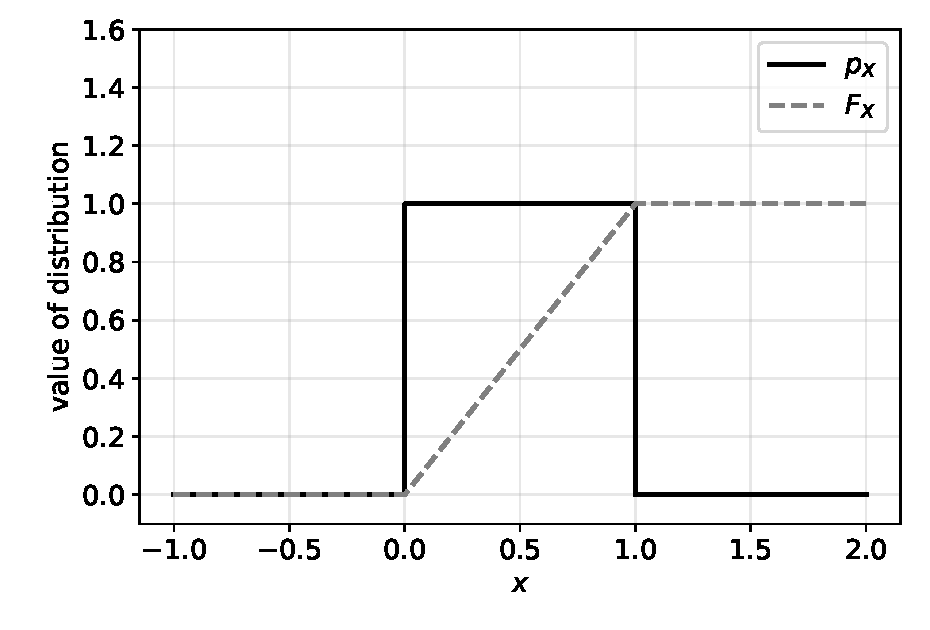
\includegraphics[width=0.62\textwidth]{fig_uniform_pdf_cdf.pdf}
\end{center}
\textbf{Plain English (figure).} The solid line is the flat pdf (density $1$
everywhere on $[0,1]$, zero outside); the dashed line is the cdf, rising
linearly from 0 to 1 across the interval --- reflecting that the probability
of landing in $[0,x]$ grows in direct proportion to $x$.
\end{frame}

\begin{frame}{Proposition 2.2.27: specifying a random variable by alphabet and probabilities}
\begin{block}{Proposition 2.2.27}
Let $\{r_i\}_{i=1}^{\infty}$ be distinct real numbers and $\{p_i\}_{i=1}^{\infty}$
a sequence with $p_i\geq 0$ and $\sum_{i=1}^{\infty}p_i=1$. Then there exists a
probability space $(\Omega,\mathcal{F},\mathrm{P})$ and random variable
$X:\Omega\to\mathbb{R}$ such that $X(\Omega)=\{r_n : n\in\mathbb{N}^+\}$ and
$\mathrm{P}(X=r_n)=p_n$ for all $n$.
\end{block}
\textbf{Plain English.} Given \emph{any} desired set of outcomes and matching
probabilities, we can always manufacture a probability space and random
variable that realizes exactly that distribution. This licenses the common
practice of specifying a random variable purely by its alphabet and
distribution, without ever mentioning the underlying sample space $\Omega$
explicitly --- as formalized in the next remark.

\begin{block}{Remark 2.2.28 (Discrete random variable via probability mass function)}
Equivalently: $X$ is simply a tuple $(\mathcal{X},p_X)$ with sample space
$\mathcal{X}$ and $p_X:\mathcal{X}\to[0,1]$ satisfying
$\sum_{x\in\mathcal{X}}p_X(x)=1$. We write $X\sim(\mathcal{X},\mathrm{P}_X)$
or simply $X\sim\mathrm{P}_X$.
\end{block}
\end{frame}

\begin{frame}[fragile]{Python: random variables, pmf and cdf from scratch}
We rebuild Example 2.2.20 (number of heads in 3 fair coin flips) purely from
its sample space, and verify Proposition 2.2.23 ($F_X(x)=\sum_{t\leq x}p_X(t)$)
numerically.
\begin{lstlisting}
import itertools

# Omega: all 8 equally likely 3-coin-flip sequences
omega = list(itertools.product("HT", repeat=3))
P = {w: 1/8 for w in omega}                 # P(A) = |A|/8

def X(w):                                   # random variable: count heads
    return w.count("H")

# Induced pmf p_X(x) = P({w : X(w) = x})
alphabet = [0, 1, 2, 3]
pX = {x: sum(P[w] for w in omega if X(w) == x) for x in alphabet}
print("pmf p_X:", pX)                       # {0: 0.125, 1: 0.375, 2: 0.375, 3: 0.125}

# cdf via Proposition 2.2.23: F_X(x) = sum_{t <= x} p_X(t)
FX = {x: sum(pX[t] for t in alphabet if t <= x) for x in alphabet}
print("cdf  F_X:", FX)                      # {0: 0.125, 1: 0.5, 2: 0.875, 3: 1.0}
\end{lstlisting}
\textbf{Output.} \texttt{pmf p\_X: \{0: 0.125, 1: 0.375, 2: 0.375, 3: 0.125\}} \\
\texttt{cdf\ \ F\_X: \{0: 0.125, 1: 0.5, 2: 0.875, 3: 1.0\}} --- matching
$\mathrm{P}(X=2)=3/8$ from Example 2.2.20 exactly.
\end{frame}

% ==========================================================================
\section{2.2.5 Joint and Conditional Probabilities}

\begin{frame}{Joint cdf, pmf, and pdf}
\begin{block}{Definition 2.2.29 (Joint cdf, pmf, pdf)}
For two random variables $X,Y$ on the same probability space, the
\emph{joint cumulative distribution function} (joint cdf) is
\[ F_{X,Y}(x,y) := \mathrm{P}(X\leq x \text{ and } Y\leq y) \]
If $X,Y$ are discrete, the \emph{joint probability mass function} (joint pmf) is
\[ p_{X,Y}(x,y) := \mathrm{P}(X=x \text{ and } Y=y) \]
\end{block}
\textbf{Plain English.} These extend the cdf/pmf to describe two random
variables \emph{simultaneously}: $F_{X,Y}(x,y)$ is the probability that $X$
is at most $x$ \emph{and} $Y$ is at most $y$, both at once.

For continuous $X,Y$, assuming suitable regularity, there is an integrable
$f:\mathbb{R}^2\to[0,\infty)$ with
$F_{X,Y}(x,y)=\int_{-\infty}^{y}\int_{-\infty}^{x}f(u,v)\,du\,dv$, and we
define the \emph{joint pdf} $p_{X,Y}(x,y):=f(x,y)$.
\end{frame}

\begin{frame}{Conditional cdf, pmf, and pdf}
\begin{block}{Definition 2.2.30 (Conditional cdf, pmf, pdf)}
\[ F_{Y|X}(y|x) = \mathrm{P}(Y\leq y \mid X=x), \qquad
\mathrm{P}(Y=y|X=x) = \frac{\mathrm{P}(Y=y,X=x)}{\mathrm{P}(X=x)} \]
\end{block}
\textbf{Plain English.} These describe the distribution of $Y$ once we
already know the exact value taken by $X$.
\end{frame}

\begin{frame}{Theorem 2.2.31: the sum rule and product rule}
\begin{block}{Theorem 2.2.31 (Sum and product rule)}
For discrete $X,Y$ with outcomes $x\in X(\Omega)$, $y\in Y(\Omega)$:
\[ \text{Sum rule:} \quad \mathrm{P}(X=x) = \sum_{y\in Y(\Omega)}\mathrm{P}(X=x,Y=y) \]
\[ \text{Product rule:} \quad \mathrm{P}(X=x,Y=y) = \mathrm{P}(X=x|Y=y)\,\mathrm{P}(Y=y) \]
For continuous $X,Y$ with pdfs $p_X,p_Y$ and joint pdf $p_{X,Y}$:
\[ \text{Sum rule:} \quad p_X(x) = \int_{-\infty}^{\infty}p_{X,Y}(x,y)\,dy
\qquad
\text{Product rule:} \quad p_{X,Y}(x,y) = p_{X|Y}(x|y)\,p_Y(y) \]
\end{block}
\textbf{Plain English.} The \emph{sum rule} says: to get the marginal (i.e.\
un-conditioned) distribution of $X$ alone, add up (or integrate out) the
joint distribution over every possible value of $Y$. The \emph{product rule}
is just Definition 2.2.13 rearranged: the joint probability of $X=x$ and
$Y=y$ equals the conditional probability of $X$ given $Y$, times the
(marginal) probability of $Y$. These also hold conditioned on a third random
variable $Z=z$, by Theorem 2.2.14.
\end{frame}

\begin{frame}{Example 2.2.32: conditional coin flips}
\begin{block}{Example 2.2.32 (Conditional coin flips)}
Recall $X=$ number of heads in 3 coin flips. Define $Y(\omega)=[\![\omega\neq TTT]\!]$
(``at least one head was flipped''). We ask: how likely is it that two heads
were flipped, given that at least one was?
\[ \mathrm{P}(X=2|Y=1) = \frac{\mathrm{P}(X=2,Y=1)}{\mathrm{P}(Y=1)} = \frac{3/8}{7/8} = \frac37 \]
\end{block}
\textbf{Plain English.} $[\![\cdot]\!]$ is the Iverson bracket: it equals 1 if
the statement inside is true, 0 otherwise. The intuition behind $3/7$:
knowing $Y=1$ rules out only the single outcome $TTT$, leaving 7 equally
likely outcomes $\{HHH,HHT,HTH,HTT,THH,THT,TTH\}$, of which exactly 3 have 2
heads.

\begin{block}{Example 2.2.34 (Dependent random variables)}
$X$ and $Y$ above are \emph{not} independent, since
$\mathrm{P}(X=0,Y=1)=\mathrm{P}(\emptyset)=0$ but
$\mathrm{P}(X=0)\mathrm{P}(Y=1) = \tfrac18\cdot\tfrac78 = \tfrac{7}{64}\neq 0$.
\end{block}
\end{frame}

\begin{frame}{Definition 2.2.33: independent and identically distributed}
\begin{block}{Definition 2.2.33 (Independent and identically distributed)}
A countable collection $(X_i)_{i\in I}$ with cdfs $\{F_{X_i}\}_{i\in I}$ are
\emph{identically distributed} if all cdfs are identical. The family
$(X_n)$ is \emph{independently distributed} (or \emph{mutually independent})
if for all finite subsets $J\subseteq I$ and all $\{x_j\}_{j\in J}$,
\[ F_{X_j : j\in J}(X_j = x_j : j\in J) = \prod_{j\in J} F_{X_j}(X_j=x_j) \]
This is stronger than \emph{pairwise independence}, which only requires
$F_{X_i,X_j}(x_i,x_j)=F_{X_i}(x_i)F_{X_j}(x_j)$ for all $i,j\in I$. If both
conditions hold, we say the family is \emph{independent and identically
distributed} (i.i.d.).
\end{block}
\textbf{Plain English.} ``Identically distributed'' means every variable in
the family follows the exact same probability law. ``Independent'' means
knowing the values of any finite subset of the variables tells you nothing
about the others --- their \emph{joint} cdf factorizes into the product of
individual cdfs. Mutual independence (all finite subsets factorize) is a
strictly stronger requirement than mere pairwise independence (only pairs
factorize).
\end{frame}

% ==========================================================================
\section{2.2.6 Expectation and Variance}

\begin{frame}{Motivating expectation via the empirical average}
Given a random variable $X$, sample outcomes $\omega_1,\omega_2,\ldots$ and
feed them into $X$ to get $X(\omega_1),X(\omega_2),\ldots$, then define the
\emph{empirical average} $\bar{X}_n:=\tfrac1n\sum_{i=1}^{n}X(\omega_i)$. For
large $n$, if $\mathrm{P}(X=x_i)=p_i$ then approximately $np_i$ of the
outcomes equal $x_i$, so
\[ \bar{X}_n \;\approx\; \frac1n\sum_{x\in X(\Omega)}(nP(X=x))\,x \;=\; \sum_{x\in X(\Omega)} x\, P(X=x) \]
\textbf{Plain English.} This heuristic argument (make it rigorous later via
the law of large numbers) motivates defining the ``theoretical average''
value of $X$ as a weighted sum of outcomes, each weighted by its probability
of occurring --- which is exactly the definition of expectation below.
\end{frame}

\begin{frame}{Definition 2.2.35: expected value}
\begin{block}{Definition 2.2.35 (Expected value)}
The \emph{expected value} (expectation, or mean) of a discrete random
variable $X$ with pmf $p(x)$ is
\[ \mathbb{E}[X] := \sum_{x\in X(\Omega)} x\, p(x) \]
For continuous $X$ with pdf $p(x)$: $\mathbb{E}[X] := \int_{-\infty}^{\infty} x\,p(x)\,dx$.
\end{block}
\textbf{Plain English.} $\mathbb{E}[X]$ (``expectation of $X$'') is the
probability-weighted average of all possible values $X$ can take. Often we
write $\sum_{x\in\mathbb{R}}$ or $\sum_x$ instead of $\sum_{x\in X(\Omega)}$,
understanding that $p(x)=0$ outside $X(\Omega)$. This sum/integral may fail
to converge, in which case $\mathbb{E}[X]$ is \emph{undefined} --- e.g.\ the
Cauchy distribution $p(x)=\tfrac1\pi\cdot\tfrac{1}{1+x^2}$ has no defined
expected value.
\end{frame}

\begin{frame}{Conditional and multi-variable expectation}
\begin{block}{Definition 2.2.36 (Conditional expectation)}
Given $X,Y$ and $g:\mathbb{R}\to\mathbb{R}$,
\[ \mathbb{E}[g(X)|Y=y] = \sum_{x\in X(\Omega)} g(x)\,p_{X|Y}(x|y)
\qquad\text{(discrete)} \]
\[ \mathbb{E}[g(X)|Y=y] = \int_{-\infty}^{\infty} g(x)\,p_{X|Y}(x|y)\,dy
\qquad\text{(continuous)} \]
\end{block}
\textbf{Plain English.} This weights the possible values of a \emph{function}
of $X$ (rather than $X$ itself) by the probability of $X$'s value
\emph{conditioned} on $Y=y$. Setting $g$ to the identity and $Y$ to a
constant recovers the unconditional $\mathbb{E}[X]$ from Definition 2.2.35.

\begin{block}{Definition 2.2.37 (Multi-variable expectation)}
For $X_1,\ldots,X_n$ with joint pmf/pdf $p_{X_1,\ldots,X_n}$ and
$f:\mathbb{R}^n\to\mathbb{R}$,
\[ \mathbb{E}[f(X_1,\ldots,X_n)] := \sum_{\mathbf{x}\in\prod_{i=1}^n X_i(\Omega_i)} f(\mathbf{x})\,p_{X_1,\ldots,X_n}(\mathbf{x}) \]
where $\mathbf{x}=(x_1,\ldots,x_n)$.
\end{block}
\end{frame}

\begin{frame}{Example 2.2.38 and Theorem 2.2.39: linearity of expectation}
\begin{block}{Example 2.2.38 (Expected value of a fair die)}
For $X$ with alphabet $\{1,\ldots,6\}$, $\mathrm{P}(x)=\tfrac16$,
\[ \mathbb{E}[X] = \sum_{x\in\{1,\ldots,6\}} \frac{x}{6} = \frac72 \]
\end{block}
\begin{block}{Theorem 2.2.39 (Expectation is linear)}
For random variables $X,Y,Z$ and scalars $a,b\in\mathbb{R}$,
\[ \mathbb{E}[aX+bY \mid Z=z] = a\,\mathbb{E}[X|Z=z] + b\,\mathbb{E}[Y|Z=z] \]
\end{block}
\textbf{Plain English.} The expectation of a scaled sum is the scaled sum of
the expectations --- true \emph{regardless} of whether $X$ and $Y$ are
independent. This is proven directly from the definition, by factoring out
the constants $a,b$ and applying the sum rule (Theorem 2.2.31) to split the
double sum over $x,y$ into two separate sums.
\end{frame}

\begin{frame}{Theorem 2.2.40: expectation of independent random variables}
\begin{block}{Theorem 2.2.40 (Expectation of independent random variables)}
If $X$ and $Y$ are independent, $\mathbb{E}[XY] = \mathbb{E}[X]\,\mathbb{E}[Y]$.
\end{block}
\textbf{Plain English.} For \emph{independent} variables (and only then, in
general) the expectation of the product equals the product of the
expectations. The converse is \emph{not} true: $\mathbb{E}[XY]=\mathbb{E}[X]\mathbb{E}[Y]$
does not imply $X,Y$ are independent.

\begin{block}{Proof}
\[ \mathbb{E}[XY] = \sum_{x,y}xy\,\mathrm{P}(X=x,Y=y) = \sum_{x,y}xy\,\mathrm{P}(X=x)\mathrm{P}(Y=y)
= \Big(\sum_x x\,\mathrm{P}(X=x)\Big)\Big(\sum_y y\,\mathrm{P}(Y=y)\Big) = \mathbb{E}[X]\mathbb{E}[Y] \]
using independence ($\mathrm{P}(X=x,Y=y)=\mathrm{P}(X=x)\mathrm{P}(Y=y)$) in
the second step, then splitting the double sum into a product of two single
sums.
\end{block}
\end{frame}

\begin{frame}{Definition 2.2.41 and Example 2.2.42: variance}
\begin{block}{Definition 2.2.41 (Variance)}
$\mathrm{Var}[X] := \mathbb{E}\big[(X-\mathbb{E}[X])^2\big]$
\end{block}
\textbf{Plain English.} Variance measures how far, on average, $X$ strays
from its own mean $\mathbb{E}[X]$, using the \emph{squared} error
$(X-\mathbb{E}[X])^2$ as the measure of distance (squaring makes positive
and negative deviations both count, and penalizes large deviations more).
Low-variance random variables concentrate their probability mass near the
mean; high-variance ones spread it further away (see the figure on the next
slide).

\begin{block}{Example 2.2.42 (Expectation and variance of a biased coin)}
For $X\in\{0,1\}$ with $\mathrm{P}(X=1)=p$, $\mathrm{P}(X=0)=1-p$:
\[ \mathbb{E}[X] = p\cdot1+(1-p)\cdot0 = p \qquad
\mathrm{Var}[X] = (1-p)(0-p)^2+p(1-p)^2 = p(1-p) \]
\end{block}
\end{frame}

\begin{frame}{Same mean, increasing variance}
\begin{center}
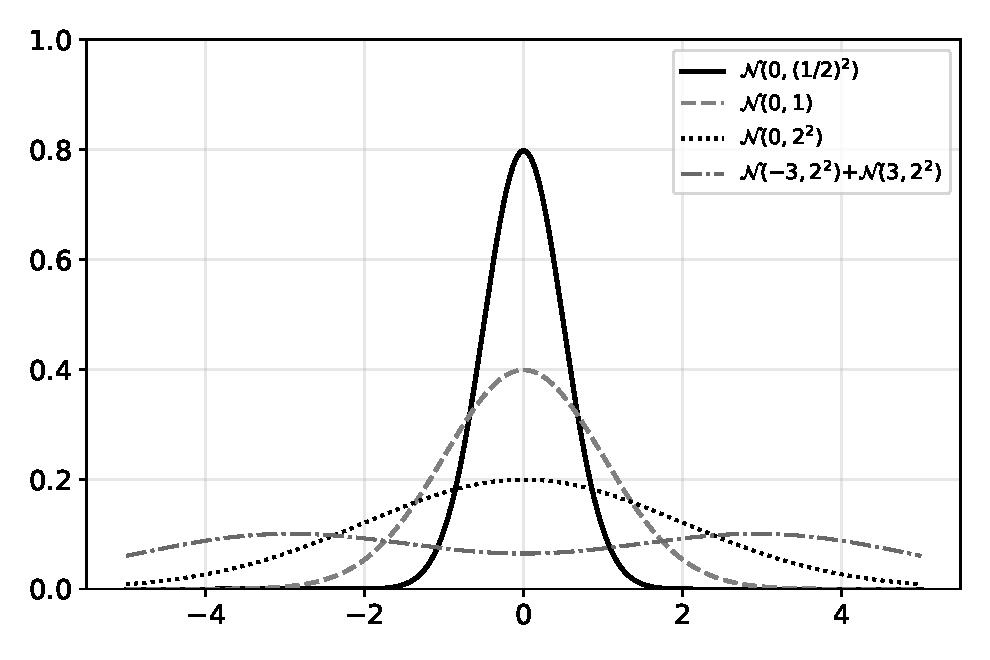
\includegraphics[width=0.62\textwidth]{fig_gaussian_variance.pdf}
\end{center}
\textbf{Plain English (figure).} Four densities, all sharing mean 0 but with
increasing spread (listed in order of increasing variance): a narrow
Gaussian, a wider Gaussian, an even wider Gaussian, and a two-humped mixture
of Gaussians centered at $\pm3$ --- the more spread out the mass, the higher
the variance. $\mathcal{N}(\mu,\sigma^2)$ (mu, sigma) denotes the Gaussian
distribution with mean $\mu$ and variance $\sigma^2$.
\end{frame}

\begin{frame}[allowframebreaks]{Theorem 2.2.43: properties of variance}
\begin{block}{Theorem 2.2.43 (Properties of variance)}
Let $X$ be a random variable, and $X_1,\ldots,X_n$ pairwise independent.
Then for any $a\in\mathbb{R}$:
\[ \mathrm{Var}[X] = \mathbb{E}[X^2]-\mathbb{E}[X]^2 \]
\[ \mathrm{Var}[aX] = a^2\,\mathrm{Var}[X] \]
\[ \mathrm{Var}[X_1+\cdots+X_n] = \mathrm{Var}[X_1]+\cdots+\mathrm{Var}[X_n] \]
\end{block}
\textbf{Plain English.} The first identity is a convenient computational
shortcut (``mean of the square minus square of the mean''). The second says
scaling a random variable by $a$ scales its variance by $a^2$ (variance has
units of ``squared'' $X$). The third --- crucially only valid for
\emph{(pairwise) independent} variables --- says variances of independent
variables simply add when the variables are summed.

\framebreak

\textbf{Proof.} \emph{(i)} Let $b=\mathbb{E}[X]$ (a constant). By linearity,
\[ \mathrm{Var}[X] = \mathbb{E}[(X-b)^2] = \mathbb{E}[X^2-2bX+b^2] = \mathbb{E}[X^2]-2b^2+b^2 = \mathbb{E}[X^2]-\mathbb{E}[X]^2 \]
\emph{(ii)} Apply (i) to $aX$:
$\mathrm{Var}[aX]=\mathbb{E}[a^2X^2]-(a\mathbb{E}[X])^2=a^2(\mathbb{E}[X^2]-\mathbb{E}[X]^2)=a^2\mathrm{Var}[X]$.
\emph{(iii)} Using $(\sum_i X_i)^2=\sum_{i,j}X_iX_j$ and (i) for $X:=\sum_i X_i$:
\[ \mathrm{Var}\Big[\sum_i X_i\Big] = \sum_{i,j}\mathbb{E}[X_iX_j] - \Big(\sum_i\mathbb{E}[X_i]\Big)^2 = \sum_{i,j}\big(\mathbb{E}[X_iX_j]-\mathbb{E}[X_i]\mathbb{E}[X_j]\big) \]
For $i\neq j$, Theorem 2.2.40 (independence) gives $\mathbb{E}[X_iX_j]-\mathbb{E}[X_i]\mathbb{E}[X_j]=0$,
so only the $i=j$ diagonal terms survive:
\[ \mathrm{Var}\Big[\sum_i X_i\Big] = \sum_{i}\big(\mathbb{E}[X_i^2]-\mathbb{E}[X_i]^2\big) = \sum_i \mathrm{Var}[X_i] \]

\begin{block}{Remark 2.2.53}
Since $x^2$ is convex, Jensen's inequality (below) gives $\mathbb{E}[X]^2\leq\mathbb{E}[X^2]$,
so $\mathrm{Var}[X]=\mathbb{E}[X^2]-\mathbb{E}[X]^2$ is always non-negative.
\end{block}
\end{frame}

% ==========================================================================
\section{2.2.7 Probability Inequalities}

\begin{frame}{Predicates, and Markov's inequality}
\begin{block}{Definition 2.2.44 and Lemma 2.2.45 (Probability of predicates)}
For a predicate $S:\Omega\to\{\text{False},\text{True}\}$, identify
$\text{False}=0$, $\text{True}=1$, and define
$\mathrm{P}(S):=\mathrm{P}(\{\omega\in\Omega:S(\omega)\})$. Then the random
variable $X(\omega)=[\![S(\omega)]\!]$ satisfies $\mathbb{E}[X]=\mathrm{P}(S)$.
\end{block}
\textbf{Plain English.} A predicate is just a True/False statement about the
outcome; treating True/False as $1/0$, the expected value of the indicator
of $S$ is exactly the probability that $S$ holds.

\begin{block}{Theorem 2.2.46 (Markov's inequality)}
If a non-negative random variable $X$ has expectation $\mathbb{E}[X]$, then
for any $\varepsilon>0$ (epsilon),
\[ \mathrm{P}(X\geq\varepsilon) \leq \frac{\mathbb{E}[X]}{\varepsilon} \]
\end{block}
\textbf{Plain English.} Markov's inequality bounds how much probability mass
can sit far out in the tail of a \emph{non-negative} random variable, using
only its mean: the chance that $X$ is at least $\varepsilon$ can never exceed
$\mathbb{E}[X]/\varepsilon$.
\end{frame}

\begin{frame}{Proof of Markov's inequality}
\begin{block}{Proof of Theorem 2.2.46}
Let $Y=\varepsilon[\![X\geq\varepsilon]\!]$. Then $Y\leq X$ always, so
$\mathbb{E}[Y]\leq\mathbb{E}[X]$. But $\mathbb{E}[Y]=\varepsilon\,\mathrm{P}(X\geq\varepsilon)$
by Lemma 2.2.45, giving $\mathrm{P}(X\geq\varepsilon)=\mathbb{E}[Y]/\varepsilon\leq\mathbb{E}[X]/\varepsilon$.
\end{block}
\textbf{Plain English.} We build an auxiliary random variable $Y$ that is
$\varepsilon$ whenever $X$ is at least $\varepsilon$, and $0$ otherwise; $Y$
never exceeds $X$, so its expectation cannot exceed $\mathbb{E}[X]$ either,
and $\mathbb{E}[Y]$ is exactly $\varepsilon$ times the probability we want to
bound.
\end{frame}

\begin{frame}{Chebyshev's inequality}
\begin{block}{Theorem 2.2.47 (Chebyshev's inequality)}
Let $X$ have finite $\mathbb{E}[X]$ and $\mathrm{Var}[X]$. Then for any
$\varepsilon>0$,
\[ \mathrm{P}(|X-\mathbb{E}[X]|\geq\varepsilon) \leq \frac{\mathrm{Var}[X]}{\varepsilon^2} \]
\end{block}
\textbf{Plain English.} Chebyshev's inequality bounds how likely $X$ is to
land far from its \emph{own} mean, using only its variance. Unlike Markov's
inequality, it needs no non-negativity assumption and bounds \emph{both}
tails of the distribution at once.

\begin{block}{Proof}
Let $Y=(X-\mathbb{E}[X])^2\geq 0$, so $\mathbb{E}[Y]=\mathrm{Var}[X]$. Apply
Markov's inequality to $\mathrm{P}(Y\geq\varepsilon^2)$:
\[ \mathrm{P}(|X-\mathbb{E}[X]|\geq\varepsilon) = \mathrm{P}((X-\mathbb{E}[X])^2\geq\varepsilon^2)
= \mathrm{P}(Y\geq\varepsilon^2) \leq \frac{\mathbb{E}[Y]}{\varepsilon^2} = \frac{\mathrm{Var}[X]}{\varepsilon^2} \]
\end{block}
\textbf{Comparing the two.} Markov's inequality only bounds the upper tail
and needs non-negativity; its bound shrinks inversely in $\varepsilon$.
Chebyshev's bounds both tails, needs no non-negativity, and its bound
shrinks inversely in $\varepsilon^2$ (i.e.\ faster).
\end{frame}

\begin{frame}[fragile]{Python: Markov and Chebyshev bounds vs.\ exact probability}
\begin{block}{Example 2.2.48 (Sum of $n$ dice)}
$S=\sum_{i=1}^n X_i$, $\mathbb{E}[S]=3.5n$. Markov: $\mathrm{P}(S\geq k)\leq \mathbb{E}[S]/k$.
For $n=20,k=80$: bound $=70/80=0.875$, true value $\approx0.1075$.
\end{block}
\begin{lstlisting}
import math
n, k = 20, 80
mu = 3.5 * n                # E[S] for n fair dice
var = n * 35 / 12           # Var[S]; Var of one die = 35/12
# Exact P(S >= k): convolve n copies of a die's pmf
dist = [1.0]                # dist[i] = P(sum of dice so far == i)
for _ in range(n):
    newdist = [0.0] * (len(dist) + 6)
    for face in range(1, 7):
        for i, p in enumerate(dist):
            newdist[i + face] += p / 6
    dist = newdist
exact  = sum(dist[k:])      # dist[i] indexes the sum value directly
markov = mu / k
cheby  = var / (k - mu) ** 2
print(f"exact={exact:.4f}  Markov<={markov:.4f}  Chebyshev<={cheby:.4f}")
\end{lstlisting}
\textbf{Output.} \texttt{exact=0.1075\ \ Markov<=0.8750\ \ Chebyshev<=0.5833}
--- both are valid upper bounds on the true value, and Chebyshev is somewhat
tighter here since it also exploits the variance of $S$.
\end{frame}

\begin{frame}{Convex and concave functions}
\begin{block}{Definition 2.2.49 (Convex function)}
$f:\mathbb{R}^n\to\mathbb{R}\cup\{\infty\}$ is \emph{convex} if for all
$x_1,x_2\in\mathbb{R}^n$ and $\theta\in[0,1]$,
\[ f(\theta x_1+(1-\theta)x_2) \leq \theta f(x_1)+(1-\theta)f(x_2) \]
(\emph{strictly} convex if the inequality is strict.)
\end{block}
\textbf{Plain English.} For $f:\mathbb{R}\to\mathbb{R}$: given any two points
$P=(x_1,f(x_1))$ and $Q=(x_2,f(x_2))$ on the graph of $f$, the straight line
segment from $P$ to $Q$ always sits \emph{above} (or on) the graph of $f$.
Examples of convex functions: $x^2$, $e^x$, $-\log(x)$, $-\sqrt{x}$.

\begin{block}{Definition 2.2.50 (Concave function)}
$f$ is \emph{concave} if the inequality reverses:
$f(\theta x_1+(1-\theta)x_2)\geq \theta f(x_1)+(1-\theta)f(x_2)$. Note $f$ is
(strictly) concave iff $-f$ is (strictly) convex.
\end{block}

\end{frame}

\begin{frame}{Lemma 2.2.51, illustrated: convexity via secants and tangents}
\begin{block}{Lemma 2.2.51 (First-order convexity conditions)}
\small
For convex $f:\mathbb{R}^n\to\mathbb{R}$, for all $x,x_0\in\mathbb{R}^n$,
$f(x) \geq f(x_0) + (x-x_0)\cdot\nabla f(x_0)$, where $\nabla$ (nabla)
denotes a sub-gradient of $f$ at $x_0$: the tangent line at any point lies
\emph{below} the function everywhere else.
\end{block}
\vspace{-1mm}
\begin{columns}[T]
\begin{column}{0.48\textwidth}
\centering
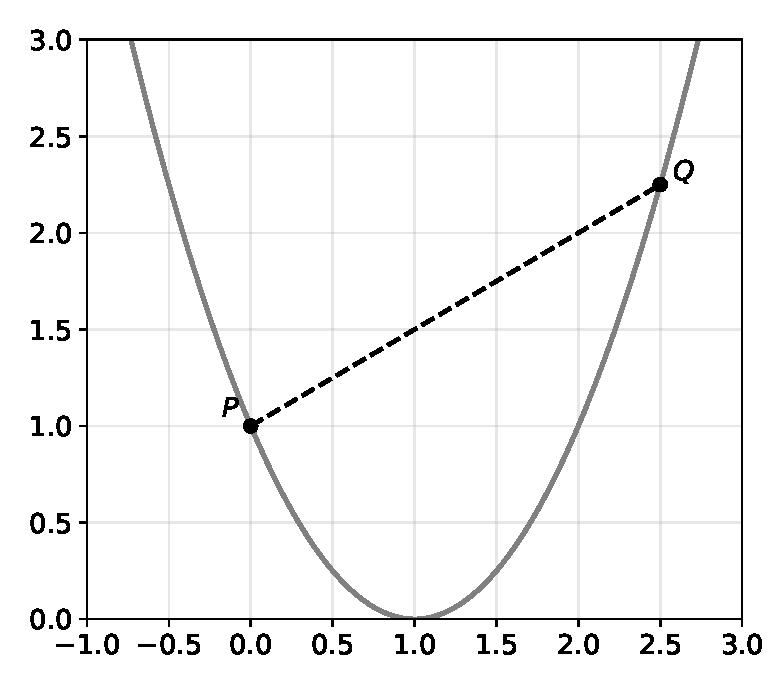
\includegraphics[width=0.72\textwidth]{fig_convex_secant.pdf}\\[-1mm]
{\scriptsize Secant $PQ$ sits \emph{above} the curve.}
\end{column}
\begin{column}{0.48\textwidth}
\centering
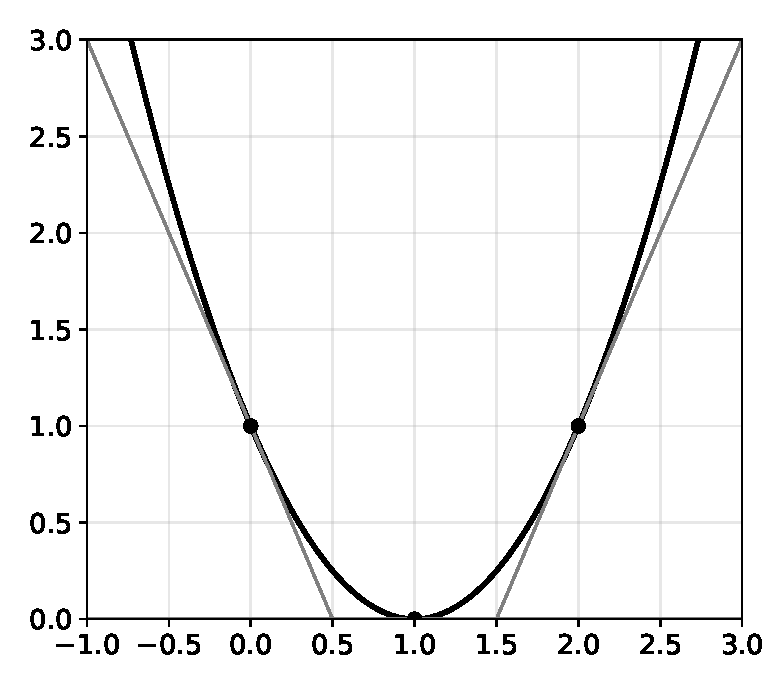
\includegraphics[width=0.72\textwidth]{fig_convex_tangent.pdf}\\[-1mm]
{\scriptsize Tangents at $x_0{=}0,1,2$ sit \emph{below} the curve.}
\end{column}
\end{columns}
\end{frame}

\begin{frame}{Theorem 2.2.52: Jensen's inequality}
\begin{block}{Theorem 2.2.52 (Jensen's inequality)}
Let $X$ be a random vector. Then
\[ f(\mathbb{E}[X]) \leq \mathbb{E}[f(X)] \quad\text{for convex } f
\qquad\qquad
g(\mathbb{E}[X]) \geq \mathbb{E}[g(X)] \quad\text{for concave } g \]
\end{block}
\textbf{Plain English.} Applying a convex function \emph{after} averaging
never overshoots applying the function \emph{first} and then averaging: the
function of the average is at most the average of the function. (For
concave functions, the inequality flips.)

\begin{block}{Proof (convex case)}
By Lemma 2.2.51 with $x_0=\mathbb{E}[X]$: $f(x)\geq f(\mathbb{E}[X])+(x-\mathbb{E}[X])\cdot\nabla f(\mathbb{E}[X])$.
Take expectations of both sides:
\[ \mathbb{E}[f(X)] \geq f(\mathbb{E}[X]) + \nabla f(\mathbb{E}[X])\cdot\underbrace{\mathbb{E}[X-\mathbb{E}[X]]}_{=0} = f(\mathbb{E}[X]) \]
(The concave case follows by applying the convex result to $-g$.)
\end{block}
\end{frame}

\begin{frame}{Corollary 2.2.54: Jensen's inequality of averages}
\begin{block}{Corollary 2.2.54 (Jensen's inequality of averages)}
Let $f$ be convex, and $(x_i)_{i=1}^n$ a finite sequence. Then
\[ f\Big(\frac1n\sum_{i=1}^n x_i\Big) \leq \frac1n\sum_{i=1}^n f(x_i) \]
\end{block}
\textbf{Plain English.} This is Jensen's inequality specialized to a uniform
average over $n$ numbers: applying convex $f$ to the plain average of the
$x_i$ never exceeds the plain average of $f(x_i)$.

\begin{block}{Proof}
Let $p=(1/n,\ldots,1/n)$ and let $X$ have sample space $\{x_1,\ldots,x_n\}$
with $\mathrm{P}(X=x_i)=1/n$. Then $\mathbb{E}[X]=\tfrac1n\sum_i x_i$ and
$\mathbb{E}[f(X)]=\tfrac1n\sum_i f(x_i)$, so Theorem 2.2.52 (Jensen's
inequality) directly gives
\[ f\Big(\frac1n\sum_i x_i\Big) = f(\mathbb{E}[X]) \leq \mathbb{E}[f(X)] = \frac1n\sum_i f(x_i) \]
\end{block}
\end{frame}

% ==========================================================================
\section{2.2.8 Convergence of Random Variables}

\begin{frame}{Motivation: what does it mean for random variables to converge?}
For an ordinary sequence of numbers $(x_n)$, ``convergence'' is unambiguous.
For a sequence of \emph{functions} $(f_n)$, there are already several
distinct notions: pointwise convergence ($\forall x, \lim_n f_n(x)=f(x)$),
uniform convergence ($\lim_n \sup_x |f_n(x)-f(x)|=0$), and $L^2$ convergence
($\lim_n\int|f_n(x)-f(x)|^2dx=0$). Since random variables are themselves
functions $\Omega\to\mathbb{R}$, we might try to directly carry across the
notion of pointwise convergence:

\begin{block}{Definition 2.2.55 (Pointwise convergence of random variables)}
$(X_n)_{n=1}^{\infty}$ converges \emph{pointwise} to $X$ if for all
$\omega\in\Omega$, $\lim_{n\to\infty}X_n(\omega)=X(\omega)$.
\end{block}
\textbf{Plain English.} This turns out to be too strong: for a ``poor''
choice of the sampled outcome $\omega$, the sequence
$\{X_n(\omega)\}_{n=1}^{\infty}$ may converge to something else entirely, or
not converge at all --- even though such $\omega$ may themselves be
extremely unlikely to ever be sampled.
\end{frame}

\begin{frame}{Example 2.2.56: pointwise (non)convergence for coin flips}
\begin{block}{Example 2.2.56 (Bernoulli pointwise (non)convergence)}
Let $X_n$ be i.i.d.\ with $\{0,1\}$ and probabilities $\{1-\theta,\theta\}$
(modelling the $n$-th flip of a biased coin). Define
$S_n(\omega_{1:\infty}) = \sum_{i=1}^n X_i(\omega_i)$ (number of 1's in the
first $n$ tosses). We would hope
\[ \forall \omega\in\Omega^\infty, \quad \lim_{n\to\infty}\frac{S_n(\omega)}{n} = \theta \]
\end{block}
\textbf{Plain English.} This says: in the long run, the fraction of heads
should settle at $\theta$. But this fails for \emph{every} choice of
$\omega$: e.g.\ for $\omega_z = 000\ldots$ (the all-zeros sequence),
$\lim_{n\to\infty}S_n(\omega_z)/n = 0 \neq \theta$. Yet we would not expect a
fair coin to actually produce an all-zeros sequence --- this particular
$\omega_z$ is simply ``unlikely''. This motivates weakening pointwise
convergence to allow a probability-zero set of exceptions.
\end{frame}

\begin{frame}{Definition 2.2.57: almost sure convergence}
\begin{block}{Definition 2.2.57 (Almost sure convergence (a.s.))}
$(X_n)_{n=1}^{\infty}$ converges \emph{almost surely} to $X$ (denoted
$X_n\xrightarrow{\text{a.s.}}X$) if
\[ \mathrm{P}\big[\{\omega\in\Omega : \lim_{n\to\infty}X_n(\omega)=X(\omega)\}\big] = 1 \]
\end{block}
\textbf{Plain English.} Rather than requiring convergence for \emph{every}
$\omega$, we only require convergence for a set of outcomes with total
probability 1 --- i.e.\ convergence happens ``almost everywhere'', ignoring a
probability-zero set of unlucky exceptions. Also called \emph{strong
convergence} or \emph{convergence with probability 1 (w.p.1)}. The set of
all counterexamples $\{\omega : X_n(\omega)\not\to X(\omega)\}$ is a
probability-zero event, so even though counterexamples may exist, we will
\emph{almost surely} never see one.
\end{frame}

\begin{frame}{Example 2.2.58: almost surely eventually flipping heads}
\begin{block}{Example 2.2.58}
For a biased coin ($0<\theta<1$), define $X_n(\omega_{1:\infty}) = [\![\exists i\leq n,\,\omega_i=1]\!]$
(``at least one head seen in the first $n$ flips''). Writing the event
$\{\omega:\exists i, \omega_i=1\}$ as the disjoint union
$\bigcup_{i=0}^{\infty}\Gamma_{0^i1}$ of cylinder sets (``$i$ zeros then a
one''),
\[ \mathrm{P}\big(\{\omega: \lim_{n\to\infty}X_n(\omega)=1\}\big) = \sum_{i=0}^{\infty}\mathrm{P}(\Gamma_{0^i1}) = \sum_{i=0}^{\infty}(1-\theta)^i\theta = \frac{\theta}{1-(1-\theta)} = 1 \]
\end{block}
\textbf{Plain English.} Since $\theta>0$, the probability of an infinite run
of all-zeros (never flipping a single head) is zero, so with probability 1
the coin eventually flips at least one head --- hence $X_n\xrightarrow{\text{a.s.}}1$.
\end{frame}

\begin{frame}{Remark 2.2.59 and the Weak Law of Large Numbers}
\begin{block}{Remark 2.2.59 (Weak law of large numbers, informally)}
For i.i.d.\ $(X_i)$ with $X=1$ w.p.\ $\theta$ and $0$ w.p.\ $1-\theta$
(a \emph{Bernoulli process}), $\mathbb{E}[X]=\theta$ and $\mathrm{Var}[X]=\theta(1-\theta)$.
Let $S_n=\sum_{i=1}^n X_i$. We can now repair Example 2.2.56: the set of
counterexample $\omega$ for which $\tfrac1n S_n(\omega)\not\to\theta$ forms a
probability-zero event.
\end{block}

\begin{center}
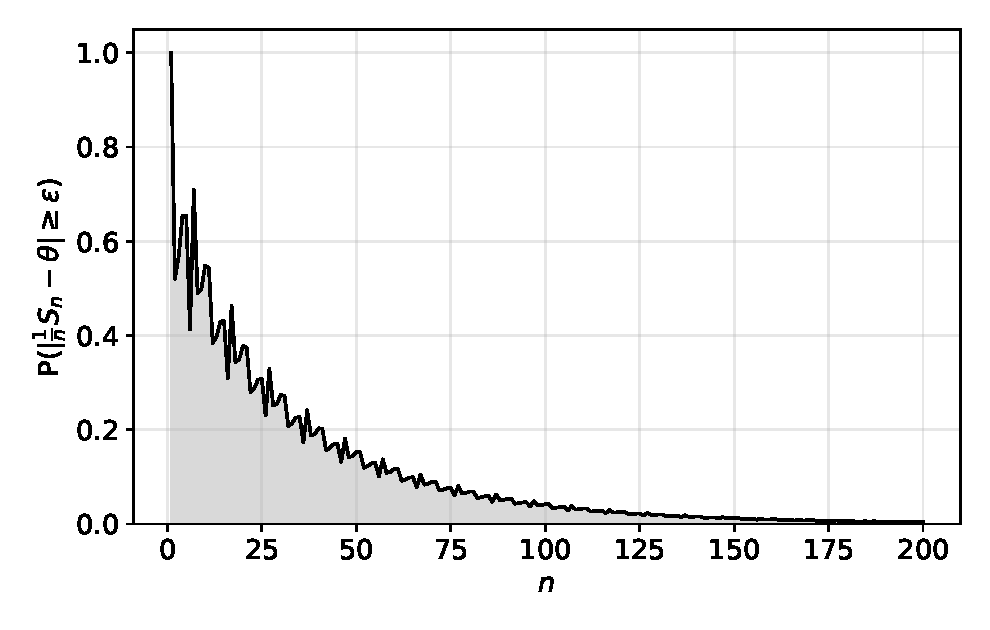
\includegraphics[width=0.58\textwidth]{fig_convergence_prob.pdf}
\end{center}
\textbf{Plain English (figure).} The exact probability
$\mathrm{P}(|\tfrac1n S_n-\theta|\geq\varepsilon)$ for $\theta=0.4$,
$\varepsilon=0.1$, plotted against $n$ (this is Figure 2.7 in the book). As
$n$ grows, this probability visibly shrinks towards zero --- the empirical
mean $\tfrac1n S_n$ concentrates ever more tightly around the true mean
$\theta$.
\end{frame}

\begin{frame}{Theorem 2.2.60: the Weak Law of Large Numbers}
\begin{block}{Theorem 2.2.60 (Weak law of large numbers)}
Let $S_n$ be a sum of $n$ i.i.d.\ Bernoulli($\theta$) random variables. Then
for all $\varepsilon>0$,
\[ \lim_{n\to\infty} \mathrm{P}\Big(\Big|\frac{S_n}{n}-\theta\Big|\geq\varepsilon\Big) = 0 \]
\end{block}
\textbf{Plain English.} The probability distribution of the sample average
$S_n/n$ concentrates \emph{all} of its probability mass onto the single
point $\theta$ as $n\to\infty$.

\begin{block}{Proof}
Let $Y=\tfrac1n S_n$. By linearity, $\mathbb{E}[Y]=\theta$, and by
Theorem 2.2.43, $\mathrm{Var}[Y] = \tfrac{1}{n^2}\sum_{i=1}^n\mathrm{Var}[X_i] = \tfrac{\theta(1-\theta)}{n}$.
By Chebyshev's inequality, and using $\theta(1-\theta)\leq\tfrac14$ for
$\theta\in[0,1]$,
\[ \mathrm{P}\Big(\Big|\frac{S_n}{n}-\theta\Big|\geq\varepsilon\Big) = \mathrm{P}(|Y-\mathbb{E}[Y]|\geq\varepsilon) \leq \frac{\mathrm{Var}[Y]}{\varepsilon^2} = \frac{\theta(1-\theta)}{\varepsilon^2 n} \leq \frac{1}{4\varepsilon^2 n} \]
which tends to 0 as $n\to\infty$.
\end{block}
\end{frame}

\begin{frame}{Theorem 2.2.61: the Hoeffding bound}
\begin{block}{Theorem 2.2.61 (Hoeffding bound)}
Let $S_n$ be a sum of $n$ independent $[0,1]$-valued random variables. Then
\[ \mathrm{P}\big(|S_n-\mathbb{E}[S_n]|\geq t\big) \leq 2e^{-2t^2/n} \]
\end{block}
\textbf{Plain English.} The proof of the weak law gave a convergence rate of
$O(n^{-1})$ (Chebyshev). Hoeffding's bound gives an \emph{exponentially}
better rate: setting $t=n\varepsilon$ for i.i.d.\ $X_i\in[0,1]$ with
$\mathbb{E}[X_i]=\theta$,
\[ \mathrm{P}\Big(\Big|\frac1n S_n-\theta\Big|\geq\varepsilon\Big) \leq 2e^{-2n\varepsilon^2} \]
which decays exponentially fast in $n$, rather than only like $1/n$.
\end{frame}

\begin{frame}{Limit supremum and limit infimum of events}
\begin{block}{Definition 2.2.62 (Limit supremum / Limit infimum)}
For a sequence of events $(A_n)_{n=1}^\infty$,
\[ \limsup_{n\to\infty}A_n := \bigcap_{n=1}^{\infty}\bigcup_{j=n}^{\infty}A_j
\qquad\qquad
\liminf_{n\to\infty}A_n := \bigcup_{n=1}^{\infty}\bigcap_{j=n}^{\infty}A_j \]
\end{block}
\begin{block}{Remark 2.2.63 (Infinitely often and almost all)}
$\omega\in\limsup A_n$ iff $\omega\in A_j$ for infinitely many $j$
(``$A_n$ infinitely often''). $\omega\in\liminf A_n$ iff $\omega\in A_j$ for
all $j$ beyond some point $n$ (``$A_n$ almost all'', i.e.\ all but finitely
many events occur).
\end{block}
\textbf{Plain English.} $\limsup A_n$ collects outcomes that keep
re-appearing in the sequence of events \emph{forever} (infinitely often,
even if not every single time); $\liminf A_n$ collects outcomes for which
\emph{eventually every subsequent event occurs} (almost all of the time,
past some point). Example 2.2.64: with the biased-coin sample space, one can
show the coin will almost surely flip a $1$ infinitely often.
\end{frame}

\begin{frame}{Convergence in probability}
\begin{block}{Definition 2.2.65 (Convergence in probability (i.p.))}
$(X_n)_{n=1}^\infty$ converges \emph{in probability} (also \emph{weak
convergence}) to $X$, denoted $X_n\xrightarrow{P}X$, if for any $\varepsilon>0$,
\[ \lim_{n\to\infty}\mathrm{P}(\{\omega\in\Omega : |X_n(\omega)-X(\omega)|>\varepsilon\}) = 0 \]
\end{block}
\textbf{Plain English.} Weaker than almost sure convergence: it only
requires the \emph{probability} of a large deviation to vanish at each fixed
$n$ (not that the sample paths themselves settle down). Theorem 2.2.60 shows
$\tfrac1n S_n\xrightarrow{P}\theta$ --- the weak law of large numbers is,
formally, an instance of convergence in probability.

\begin{block}{Theorem 2.2.66 (Convergence a.s.\ implies convergence i.p.)}
If $X_n\xrightarrow{\text{a.s.}}X$, then $X_n\xrightarrow{P}X$.
\end{block}
\textbf{Plain English.} Almost sure convergence is \emph{strictly stronger}
than convergence in probability: it implies i.p.\ convergence, but --- as
Example 2.2.67 shows next --- the converse fails. This is why almost sure
convergence is called ``strong'' and convergence in probability is called
``weak''.
\end{frame}

\begin{frame}{The convergence hierarchy (Figure 2.8)}
\begin{center}
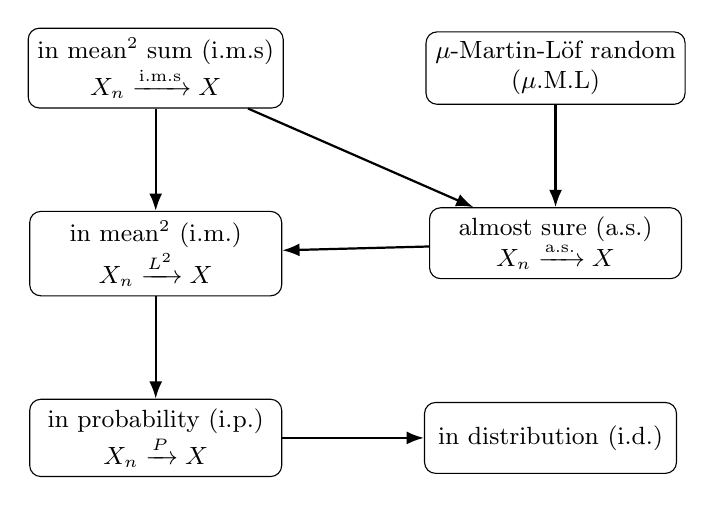
\begin{tikzpicture}[
  node distance=13mm and 18mm,
  box/.style={draw, rounded corners, align=center, minimum width=32mm, minimum height=9mm, font=\small},
  ar/.style={-{Latex[length=2.2mm]}, thick}
]
\node[box] (ims)  {in mean$^2$ sum (i.m.s)\\$X_n\xrightarrow{\text{i.m.s}}X$};
\node[box, right=of ims] (mml) {$\mu$-Martin-L\"of random\\($\mu$.M.L)};
\node[box, below=of ims] (im)  {in mean$^2$ (i.m.)\\$X_n\xrightarrow{L^2}X$};
\node[box, below=of mml] (as)  {almost sure (a.s.)\\$X_n\xrightarrow{\text{a.s.}}X$};
\node[box, below=of im]  (ip)  {in probability (i.p.)\\$X_n\xrightarrow{P}X$};
\node[box, right=of ip]  (id)  {in distribution (i.d.)};

\draw[ar] (ims) -- (im);
\draw[ar] (ims) -- (as);
\draw[ar] (mml) -- (as);
\draw[ar] (im)  -- (ip);
\draw[ar] (as)  -- (im);
\draw[ar] (ip)  -- (id);
\end{tikzpicture}
\end{center}
\textbf{Plain English.} An arrow $A\to B$ means ``$A$-convergence implies
$B$-convergence''. Convergence in mean$^2$ sum is the strongest notion
shown; convergence in distribution is the weakest. Notably, almost sure
convergence and convergence in mean$^2$ each imply convergence in
probability, but neither is implied by it (as the next example shows).
\end{frame}

\begin{frame}[allowframebreaks]{Example 2.2.67: convergence i.p.\ does not imply convergence a.s.}
\begin{block}{Example 2.2.67}
On $\Omega=[0,1]$ (Example 2.2.25), define binary intervals
\[ I_{2^m+i} = \Big[\frac{i}{2^m},\frac{i+1}{2^m}\Big), \qquad m=0,1,2,\ldots,\ i=0,\ldots,2^m-1 \]
For each $m$ there are $2^m$ intervals of length $2^{-m}$ covering $[0,1]$.
As $m\to\infty$, $\mathrm{P}(I_n)=\mathrm{P}(I_{2^m})=2^{-m}\to 0$. Define
$Y_n(\omega) = [\![\omega\in I_n]\!]$.
\end{block}

\begin{center}
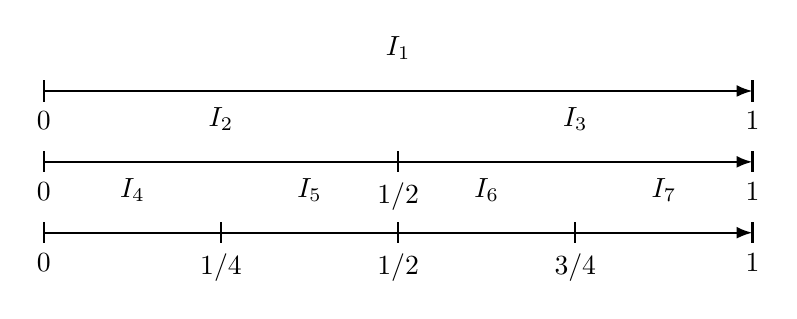
\begin{tikzpicture}[scale=0.9]
\draw[thick,-{Latex[length=2mm]}] (0,2) -- (10,2);
\draw[thick] (0,2.15) -- (0,1.85) node[below] {0};
\draw[thick] (10,2.15) -- (10,1.85) node[below] {1};
\node[above] at (5,2.3) {$I_1$};

\draw[thick,-{Latex[length=2mm]}] (0,1) -- (10,1);
\draw[thick] (0,1.15) -- (0,0.85) node[below] {0};
\draw[thick] (5,1.15) -- (5,0.85) node[below] {$1/2$};
\draw[thick] (10,1.15) -- (10,0.85) node[below] {1};
\node[above] at (2.5,1.3) {$I_2$};
\node[above] at (7.5,1.3) {$I_3$};

\draw[thick,-{Latex[length=2mm]}] (0,0) -- (10,0);
\draw[thick] (0,0.15) -- (0,-0.15) node[below] {0};
\draw[thick] (2.5,0.15) -- (2.5,-0.15) node[below] {$1/4$};
\draw[thick] (5,0.15) -- (5,-0.15) node[below] {$1/2$};
\draw[thick] (7.5,0.15) -- (7.5,-0.15) node[below] {$3/4$};
\draw[thick] (10,0.15) -- (10,-0.15) node[below] {1};
\node[above] at (1.25,0.3) {$I_4$};
\node[above] at (3.75,0.3) {$I_5$};
\node[above] at (6.25,0.3) {$I_6$};
\node[above] at (8.75,0.3) {$I_7$};
\end{tikzpicture}
\end{center}
\textbf{Plain English (figure, Figure 2.9 in book).} At level $m$, the unit
interval is chopped into $2^m$ equal binary sub-intervals $I_{2^m},\ldots,I_{2^{m+1}-1}$;
as $m$ grows, each individual sub-interval shrinks to length $2^{-m}$, so its
probability under the uniform measure shrinks to 0.

\framebreak

For any $0<\varepsilon\leq1$,
\[ \lim_{n\to\infty}\mathrm{P}(|Y_n-0|>\varepsilon) = \lim_{n\to\infty}\mathrm{P}(Y_n=1) = \lim_{n\to\infty}\mathrm{P}(I_n)=0 \]
so $Y_n\xrightarrow{P}0$. \textbf{However}, $Y_n\not\xrightarrow{\text{a.s.}}0$:
for \emph{every} $\omega\in[0,1)$, since $I_{2^m},\ldots,I_{2^{m+1}-1}$
partitions $[0,1)$ at every level $m$, $\omega$ belongs to exactly one
interval at each level, so $Y_n(\omega)=1$ infinitely often (once per level
$m$), and the limit $\lim_{n\to\infty}Y_n(\omega)$ never settles --- it
diverges for \emph{every} $\omega$:
\[ \mathrm{P}\big(\{\omega\in\Omega : \lim_{n\to\infty}Y_n(\omega)=0\}\big) = \mathrm{P}(\emptyset) = 0 \neq 1 \]
\textbf{Plain English.} This is the promised counterexample: convergence in
probability holds (the probability of a deviation shrinks to 0 with $n$),
yet almost sure convergence completely fails (in fact, \emph{every} sample
path fails to converge) --- confirming that i.p.\ is strictly weaker than a.s.
\end{frame}

\begin{frame}[allowframebreaks]{Convergence in mean$^2$ and in mean$^2$ sum}
\begin{block}{Definition 2.2.69 (Convergence in mean$^2$ (i.m.))}
$(X_n)$ converges \emph{in mean$^2$} to $X$ (denoted $X_n\xrightarrow{L^2}X$)
if $\lim_{n\to\infty}\mathbb{E}[(X_n-X)^2]=0$. (``Mean$^2$'' is pronounced
``in mean square''; not a footnote superscript.)
\end{block}
\begin{block}{Proposition 2.2.70 (Convergence in mean$^2$ implies convergence in probability)}
If $X_n\xrightarrow{L^2}X$, then $X_n\xrightarrow{P}X$.
\end{block}
\textbf{Proof.} By Markov's inequality applied to $|X_n-X|^2$:
\[ \mathrm{P}(|X_n-X|>\varepsilon) = \mathrm{P}(|X_n-X|^2>\varepsilon^2) \leq \frac{1}{\varepsilon^2}\mathbb{E}[|X_n-X|^2] \longrightarrow 0 \]

\begin{block}{Example 2.2.71 (i.p.\ does not imply i.m.)}
Let $X_n=n$ w.p.\ $1/n$, else $0$. Then $\mathrm{P}(|X_n|>\varepsilon)=1/n\to0$
so $X_n\xrightarrow{P}0$, but $\mathbb{E}[X_n^2]=n^2\cdot\tfrac1n=n\to\infty$,
so $X_n\not\xrightarrow{L^2}0$.
\end{block}

\framebreak

\begin{block}{Definition 2.2.72 (Convergence in mean$^2$ sum (i.m.s))}
$(X_n)_{n=1}^\infty$ (non-negative) converges \emph{in mean$^2$ sum} to $X$
if $\sum_{n=1}^{\infty}\mathbb{E}[(X_n-X)^2] < \infty$.
\end{block}
\begin{block}{Proposition 2.2.73 (Conv.\ in mean$^2$ sum implies conv.\ in mean$^2$)}
Trivial: an infinite sum of non-negative terms can only be finite if the
summands themselves tend to zero.
\end{block}
\textbf{Plain English.} Convergence in mean$^2$ sum is a strictly stronger
notion: not only must $\mathbb{E}[(X_n-X)^2]\to0$, but these quantities must
shrink \emph{fast enough} that their infinite sum stays finite.
\end{frame}

\begin{frame}{Borel-Cantelli Lemma, and convergence i.m.s.\ implies a.s.}
\begin{block}{Lemma 2.2.74 (Borel-Cantelli)}
If $\sum_{n=1}^{\infty}\mathrm{P}(E_n) < \infty$, then
$\mathrm{P}(\limsup_{n\to\infty}E_n)=0$: the probability that infinitely many
of $E_1,E_2,\ldots$ occur is zero.
\end{block}
\textbf{Plain English.} If the probabilities of a sequence of events shrink
fast enough to sum to something finite, then (almost surely) only
\emph{finitely many} of those events can ever actually happen.

\begin{block}{Theorem 2.2.75 (Convergence i.m.s.\ implies convergence a.s.)}
If $X_n\xrightarrow{\text{i.m.s}}X$, then $X_n\xrightarrow{\text{a.s.}}X$.
\end{block}
\textbf{Proof sketch.} Let $Y_n=X_n-X$ and $E_n=\{\omega : Y_n(\omega)^2\geq\varepsilon^2\}$.
By Markov's inequality, $\mathrm{P}(E_n)\leq\mathbb{E}[Y_n^2]/\varepsilon^2$, so
$\sum_n \mathrm{P}(E_n)\leq\tfrac{1}{\varepsilon^2}\sum_n\mathbb{E}[Y_n^2]<\infty$
by the i.m.s.\ assumption. Borel-Cantelli then gives
$\mathrm{P}(\limsup_n E_n)=0$, which (unpacking Definition 2.2.57(ii)) is
exactly almost sure convergence $Y_n\xrightarrow{\text{a.s.}}0$, i.e.\
$X_n\xrightarrow{\text{a.s.}}X$.
\end{frame}

\begin{frame}[fragile]{Python: simulating the weak law of large numbers and Hoeffding's bound}
We simulate a biased coin and empirically check the gap between Chebyshev's
($O(1/n)$) and Hoeffding's (exponential) tail bounds.
\begin{lstlisting}
import random, math
theta, eps, trials = 0.4, 0.1, 200_000
def deviation_freq(n):
    """Empirical P(|S_n/n - theta| >= eps) over `trials` runs."""
    bad = 0
    for _ in range(trials):
        S = sum(1 for _ in range(n) if random.random() < theta)
        if abs(S / n - theta) >= eps:
            bad += 1
    return bad / trials
for n in [50, 150, 300]:
    empirical = deviation_freq(n)
    chebyshev = min(1.0, theta * (1 - theta) / (eps ** 2 * n))
    hoeffding = min(1.0, 2 * math.exp(-2 * n * eps ** 2))
    print(f"n={n:4d}  empirical={empirical:.4f}"
          f"  Chebyshev<={chebyshev:.4f}  Hoeffding<={hoeffding:.4f}")
\end{lstlisting}
\textbf{Typical output.} \texttt{n=50\ \ empirical=0.1533\ \ Chebyshev<=0.4800\ \ Hoeffding<=0.7358};
\texttt{n=300\ empirical=0.0003\ \ Chebyshev<=0.0800\ \ Hoeffding<=0.0050}
--- both bounds stay valid, and Hoeffding decays exponentially faster, as
Theorem 2.2.61 predicts.
\end{frame}

% ==========================================================================
\section{Summary}

\begin{frame}{Chapter 2.2 summary}
\begin{itemize}
\item \textbf{Foundations (2.2.1--2.2.2).} A $\sigma$-algebra $\mathcal{F}$
picks out which subsets of $\Omega$ count as measurable ``events''; a
probability (semi)measure $\mathrm{P}$ assigns them numbers in $[0,1]$
satisfying countable additivity. Cylinder sets $\Gamma_x$ and (semi)measures
$\nu$ on $\mathcal{X}^\infty$ are the central objects used throughout the
rest of the book.
\item \textbf{Conditioning and random variables (2.2.3--2.2.5).} Conditional
probability $\mathrm{P}(B|A)$ restricts attention to $A$; a random variable
$X:\Omega\to\mathbb{R}$ turns outcomes into numbers, inducing a cdf/pmf/pdf;
joint and conditional distributions extend this to several variables at
once, governed by the sum and product rules.
\item \textbf{Expectation, variance, inequalities (2.2.6--2.2.7).}
$\mathbb{E}[X]$ is the probability-weighted average; $\mathrm{Var}[X]$
measures spread around it; Markov, Chebyshev, and Jensen's inequalities
bound tail probabilities and convex transformations using only these
summary statistics.
\item \textbf{Convergence (2.2.8).} Random variables can converge to a limit
in several inequivalent senses --- almost surely, in probability, in mean$^2$,
in mean$^2$ sum, in distribution --- forming a strict hierarchy
(Figure 2.8). The weak law of large numbers and the exponentially sharper
Hoeffding bound both formalize ``sample averages concentrate around the true
mean'' as $n\to\infty$.
\end{itemize}
\end{frame}

\end{document}
